\documentclass{article}
%\usepackage{tex4ht}
\usepackage{amsmath}
\usepackage{amsfonts}
\usepackage{amssymb}
\usepackage{amsthm}
\usepackage{graphicx}
\usepackage{color}
\usepackage{float}
\usepackage{dsfont}
\setlength{\parskip}{0.5\baselineskip}
\author{Zhuo Liu (0983311)}
\title{Project on Automatic Learning (Phase 1)}
\date{February 12, 2014}

\definecolor{lightgray}{gray}{0.5}


\begin{document}
\maketitle


\section{Introduction}

The goal for the project is to build a classification model learning from training set and test the accuracy by test set. 
The method we use to build the model is SVM (support vector machine). However, before building this model, we need first do a preprocessing
procedure on the data, which are PCA and kernel PCA. We will compare the results obtained by these two methods.
This project is composed by 3 phases:

\noindent Phase 1: Introduce the database we choose (one large and one small).

\noindent Phase 2: Use PCA and kernel PCA to preprocess the data, and use maximum-likelihood method based on the results from kernel PCA to build
                   a gaussian linear classifier and test it.

\noindent Phase 3: Use SVM to build classification model and test the model.

%%% ------------------------------------------------------------------------------
\goodbreak

\section{Database: the Large One}

The title of this database is ``Semeion Handwritten Digit''. 1593 handwritten digits from around 80 persons were scanned, stretched in 
a rectangular box 16x16 in a gray scale of 256 values. Then each pixel of each image was scaled into a boolean (1/0) value using a fixed threshold.

Each person wrote on a paper all the digits from 0 to 9, twice. The commitment was to write the digit the first time in the normal way 
(trying to write each digit accurately) and the second time in a fast way (with no accuracy).

Hence, this dataset consists of 1593 records (rows) ,256 attributes (columns) and 10 classes (0-9).

Each record represents a handwritten digit, orginally scanned with a resolution of 256 grays scale (28).

Each pixel of the each original scanned image was first stretched, and after scaled between 0 and 1 (setting to 0 every pixel whose value was 
under tha value 127 of the grey scale (127 included) and setting to 1 each pixel whose orinal value in the grey scale was over 127).

Finally, each binary image was scaled again into a 16x16 square box (the final 256 binary attributes). 

The following graphs are the distributions for frequency on 1 and frequency on 0 and the corresponding ratio for each attribute, then the frequencies
for each class.

\begin{figure}[htp]
\centering
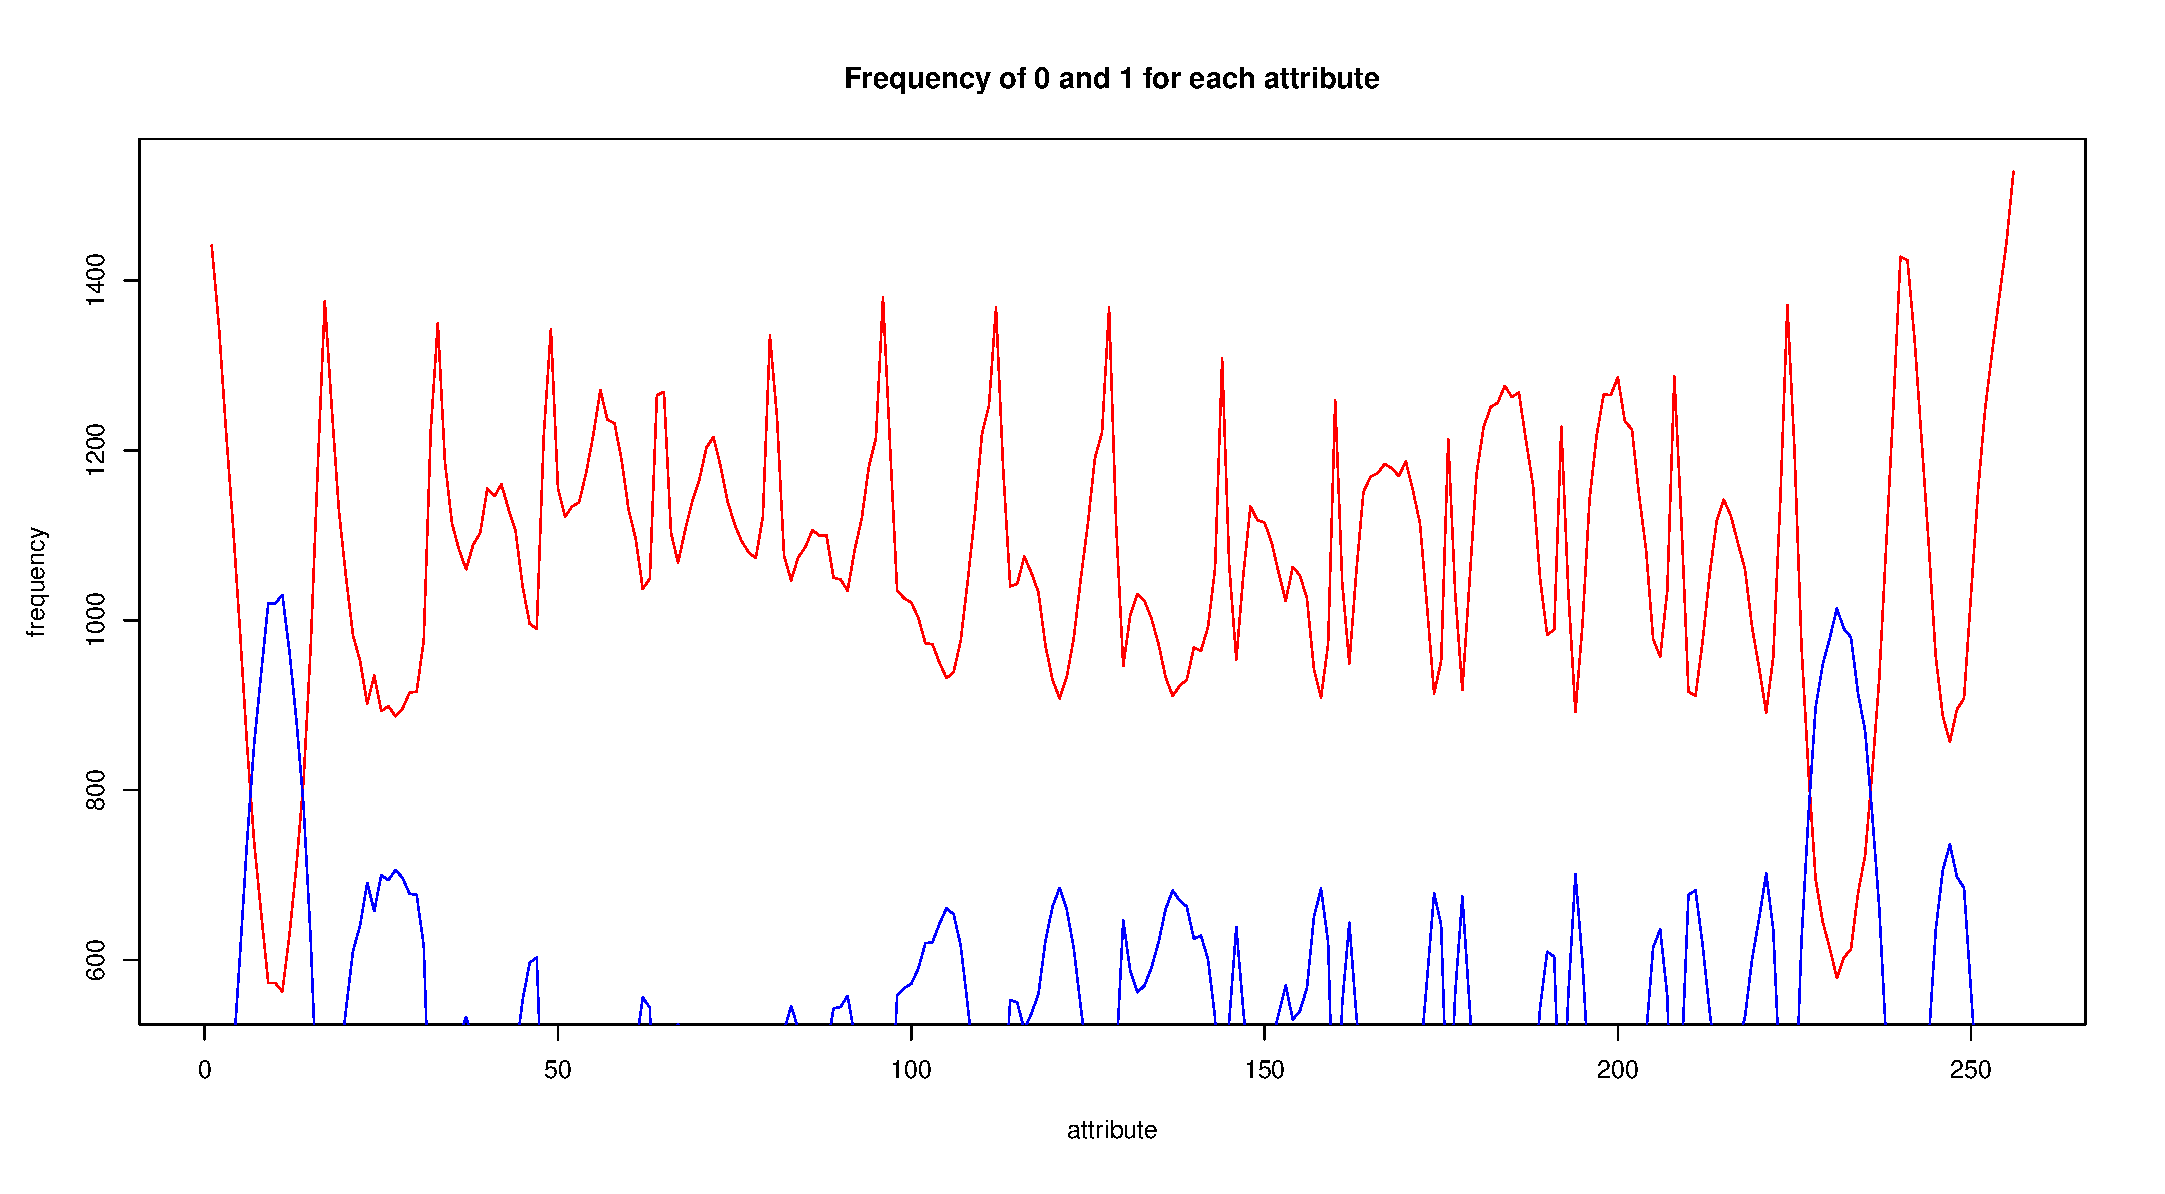
\includegraphics[width=11.3cm]{freq.eps}
\caption{Frequencies of 1 and 0 (blue=1, red=0) for each attribute}
\end{figure}

\begin{figure}[htp]
\centering
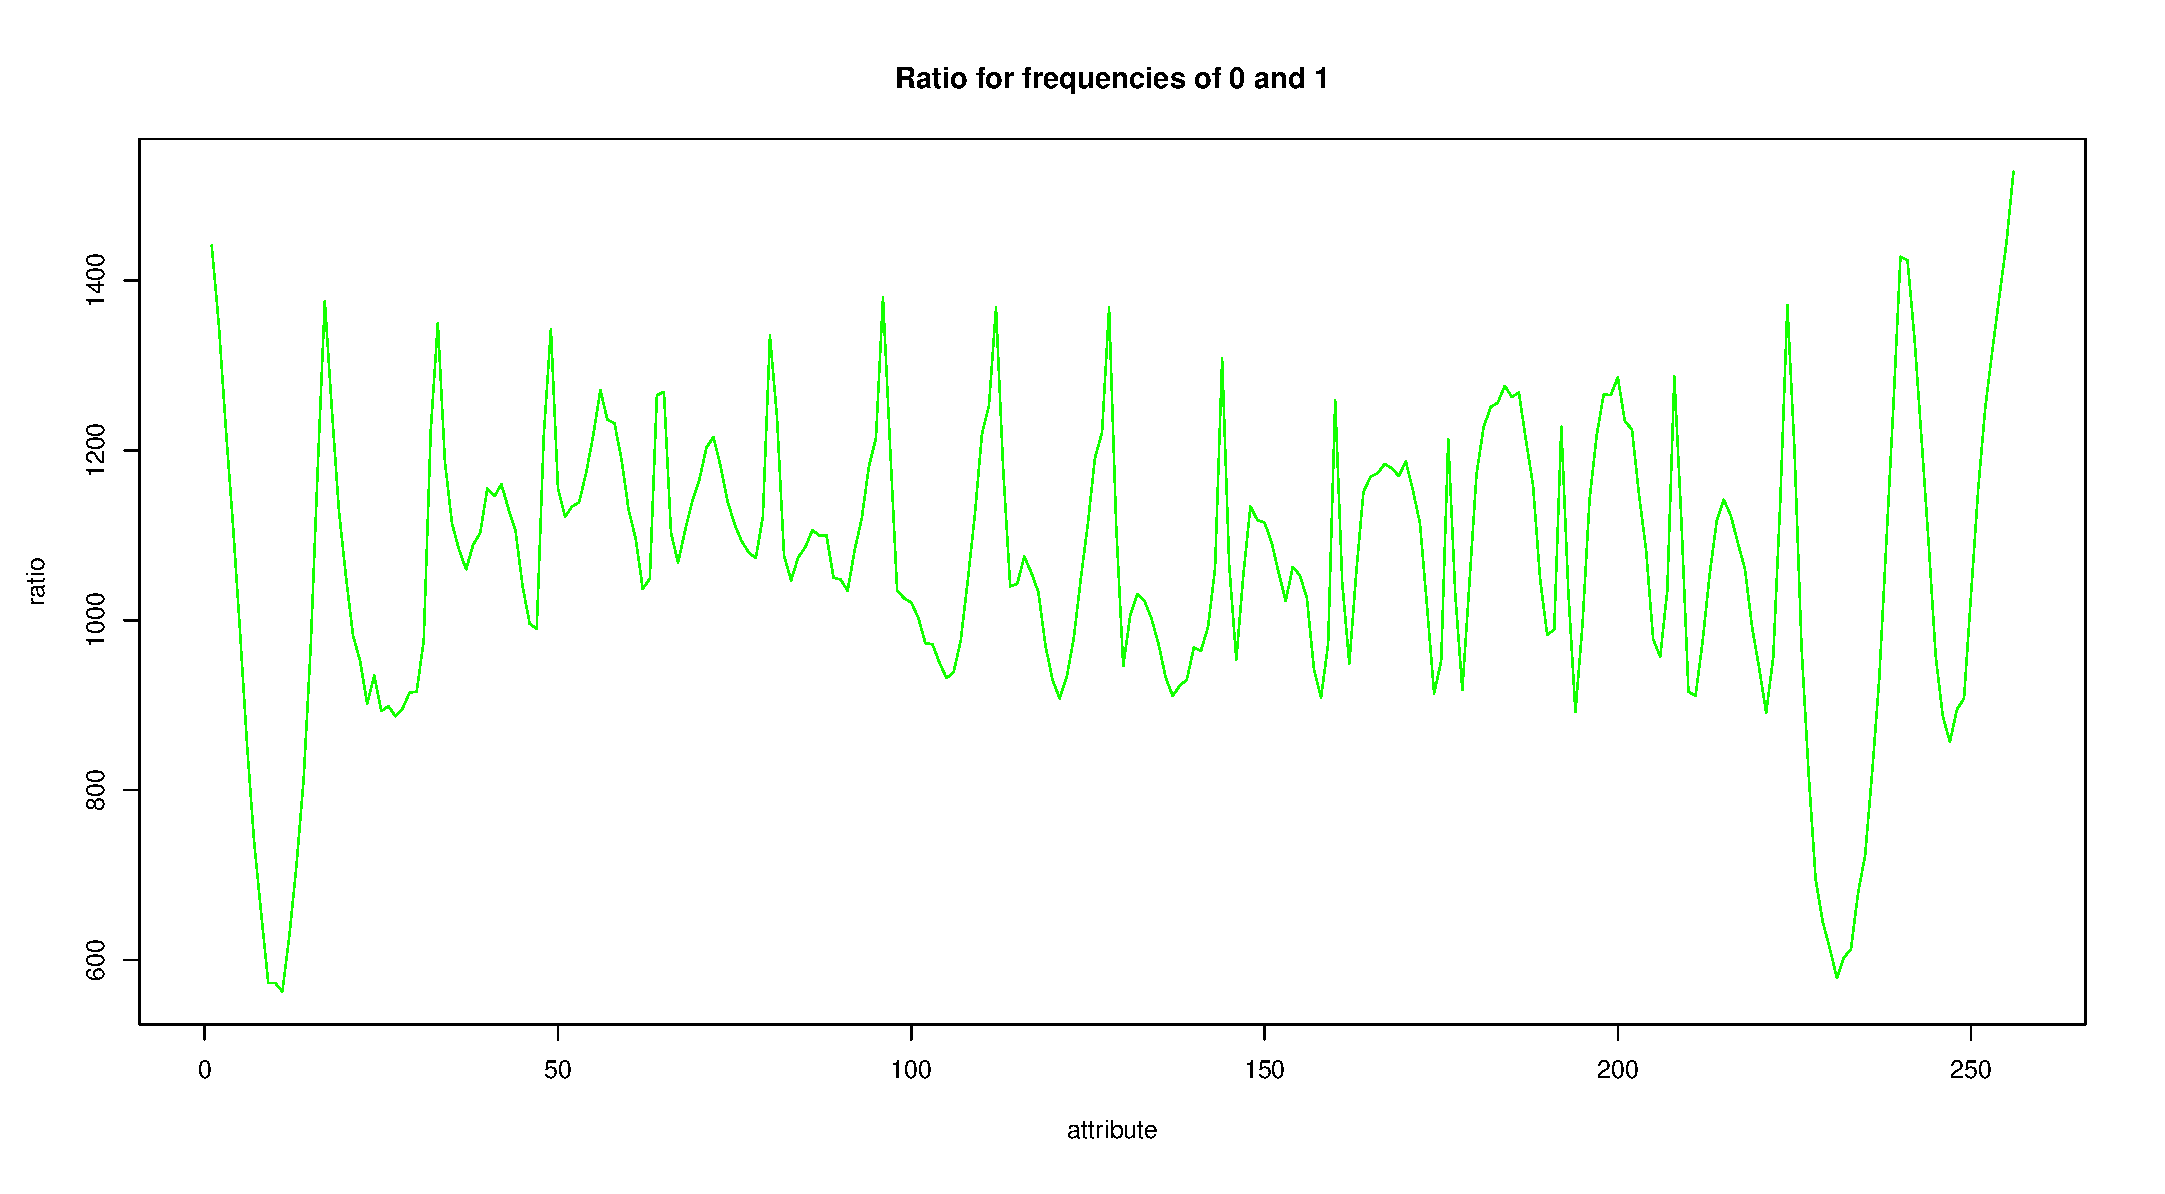
\includegraphics[width=11.3cm]{ratio.eps}
\caption{Ratio $\frac{freq(0)}{freq(1)}$ for each attribute}
\end{figure}

\begin{figure}[htp]
\centering
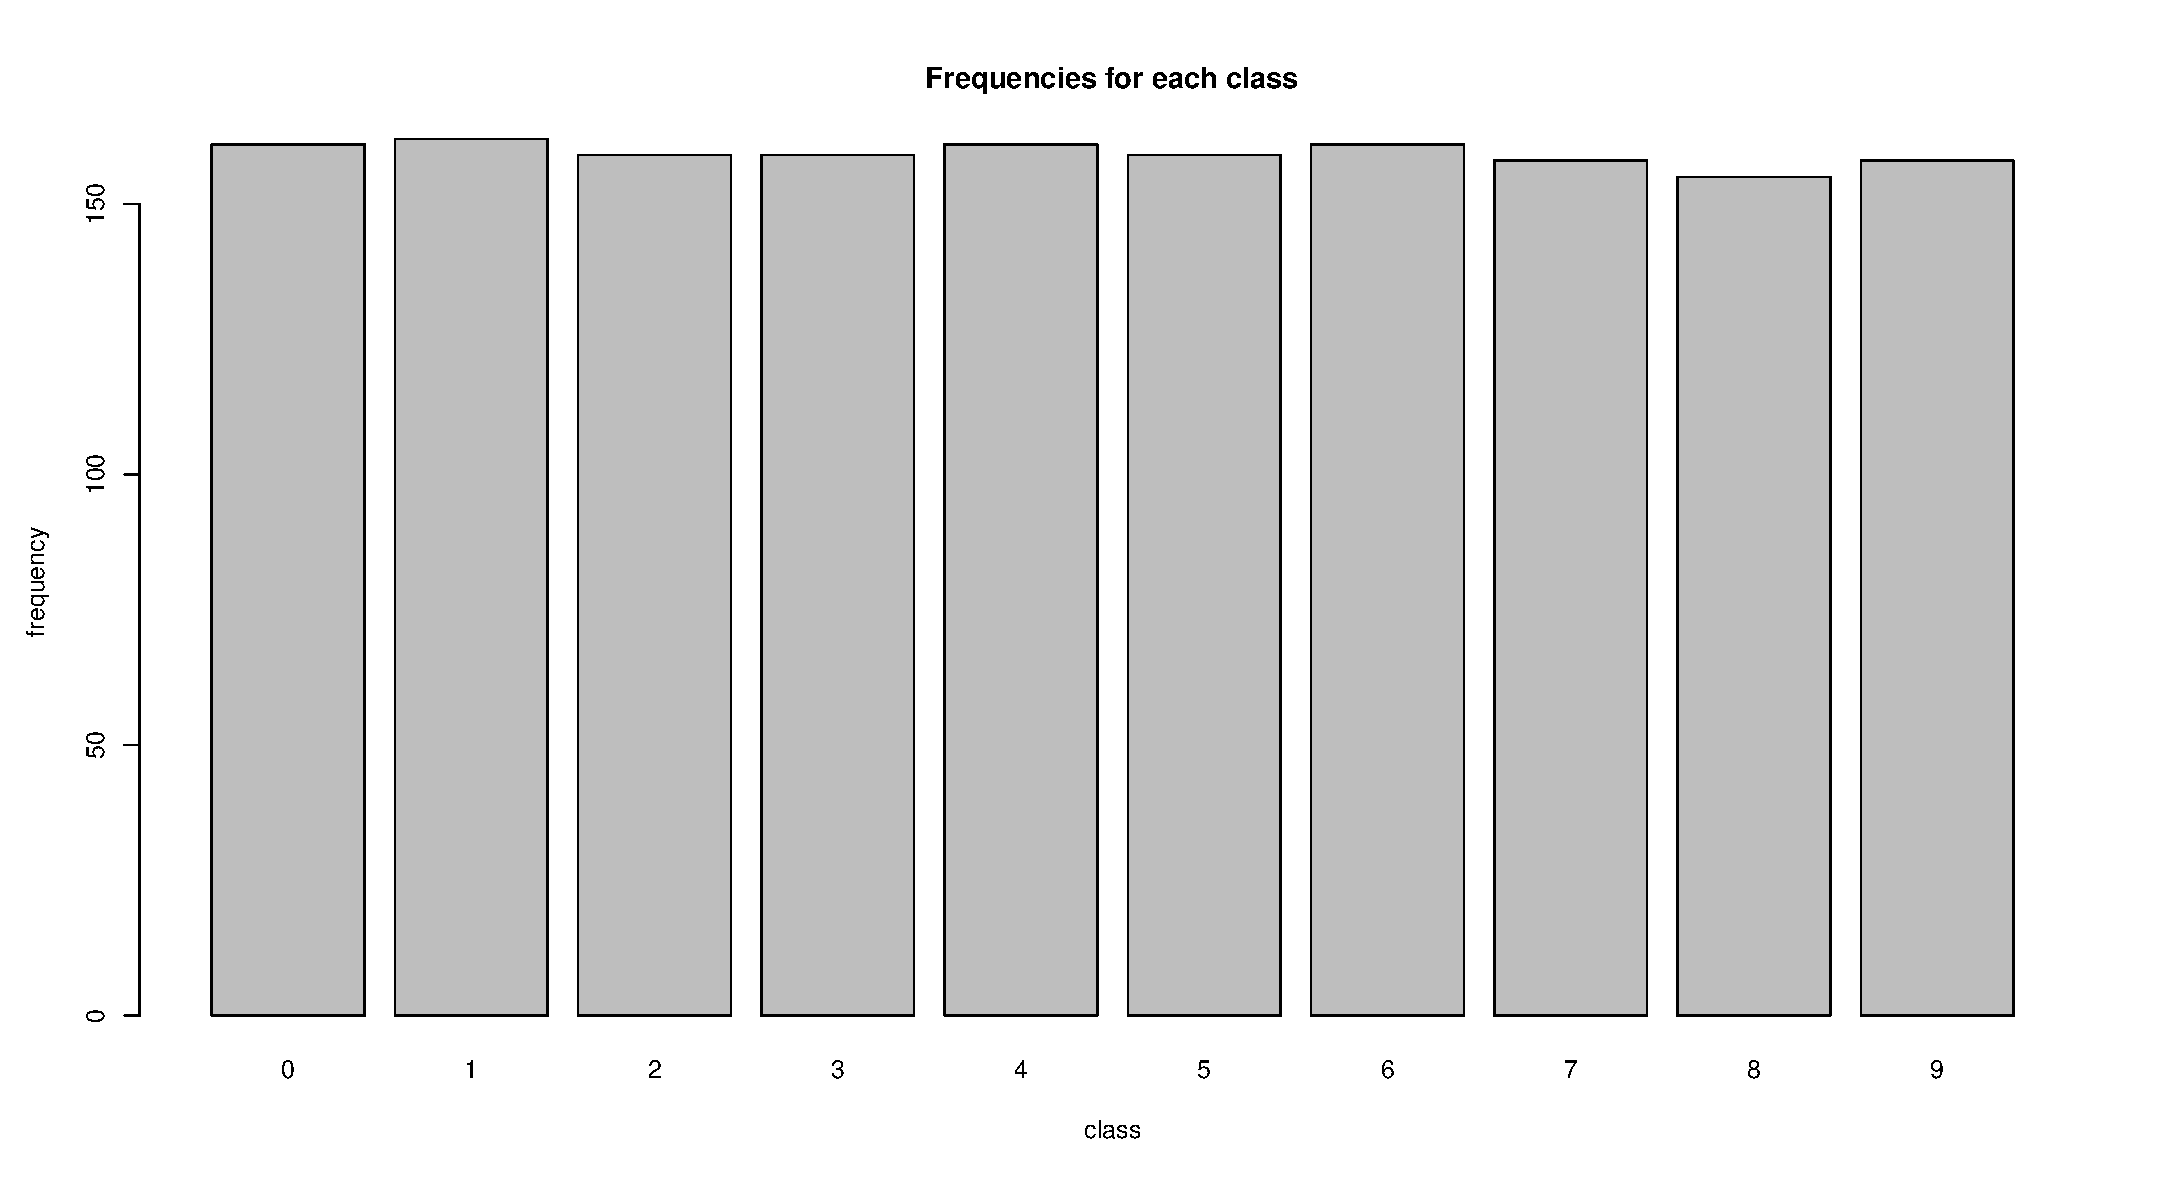
\includegraphics[width=11.3cm]{bclass.eps}
\end{figure}


%%% ------------------------------------------------------------------------------
\goodbreak

\section{Database: the Small One}

The title of this database is ``Image Segmentation'', which contains the information of pixels of outdoor images, which are labeled into 7 
classes (brickface, sky, foliage, cement, window, path, grass).

The number of instances is 2320, and the number of attributes (all continuous real numbers) is 19. The following is the information about 
attributes (The intervals after the names of attributes are the ranges, however, I cannot find the units from README file):
    
    1.  region-centroid-col (1 to 254):  the column of the center pixel of the region.
    
    2.  region-centroid-row (11 to 251):  the row of the center pixel of the region.
    
    3.  region-pixel-count (all 9):  the number of pixels in a region = 9.
    
    4.  short-line-density-5 (0 to $\frac{1}{3}$):  the results of a line extractoin algorithm that counts how many lines of length 5 (any orientation) with
        low contrast, less than or equal to 5, go through the region.
        
    5.  short-line-density-2 (0 to $\frac{2}{9}$):  same as short-line-density-5 but counts lines of high contrast, greater than 5.
    
    6.  vedge-mean (0 to 29.22222):  measure the contrast of horizontally adjacent pixels in the region.  There are 6, the mean and standard deviation are given.  
        This attribute is used as a vertical edge detector.
        
    7.  vegde-sd (0 to 991.7184):  (see 6)
    
    8.  hedge-mean (0 to 44.72223):  measures the contrast of vertically adjacent pixels. Used for horizontal line detection. 
    
    9.  hedge-sd (-1.589457e-08 to 1.386329e+03): (see 8).
    
    10. intensity-mean (0 to 143.4444):  the average over the region of (R + G + B)/3
    
    11. rawred-mean (0 to 137.1111): the average over the region of the R value.
    
    12. rawblue-mean (0 to 150.8889): the average over the region of the B value.
    
    13. rawgreen-mean (0 to 142.5556): the average over the region of the G value.
    
    14. exred-mean (-49.666668 to 9.888889): measure the excess red:  (2R - (G + B))
    
    15. exblue-mean: measure the excess blue (-12.44444 to 82):  (2B - (G + R))
    
    16. exgreen-mean: measure the excess green (-33.88889 to 24.66667):  (2G - (R + B))
    
    17. value-mean:  3-d nonlinear transformation of RGB (0 to 150.8889). (Algorithm can be found in Foley and VanDam, Fundamentals of Interactive Computer 
        Graphics)
        
    18. saturatoin-mean (0 to 1):  (see 17)
    
    19. hue-mean (-3.044175 to 2.912480):  (see 17)
    
The following are the graph for proportion of each class, and the histograms on each attribute for different classes (except ``region-pixel-count'', 
because all the values are 9).

\begin{figure}[htp]
\centering
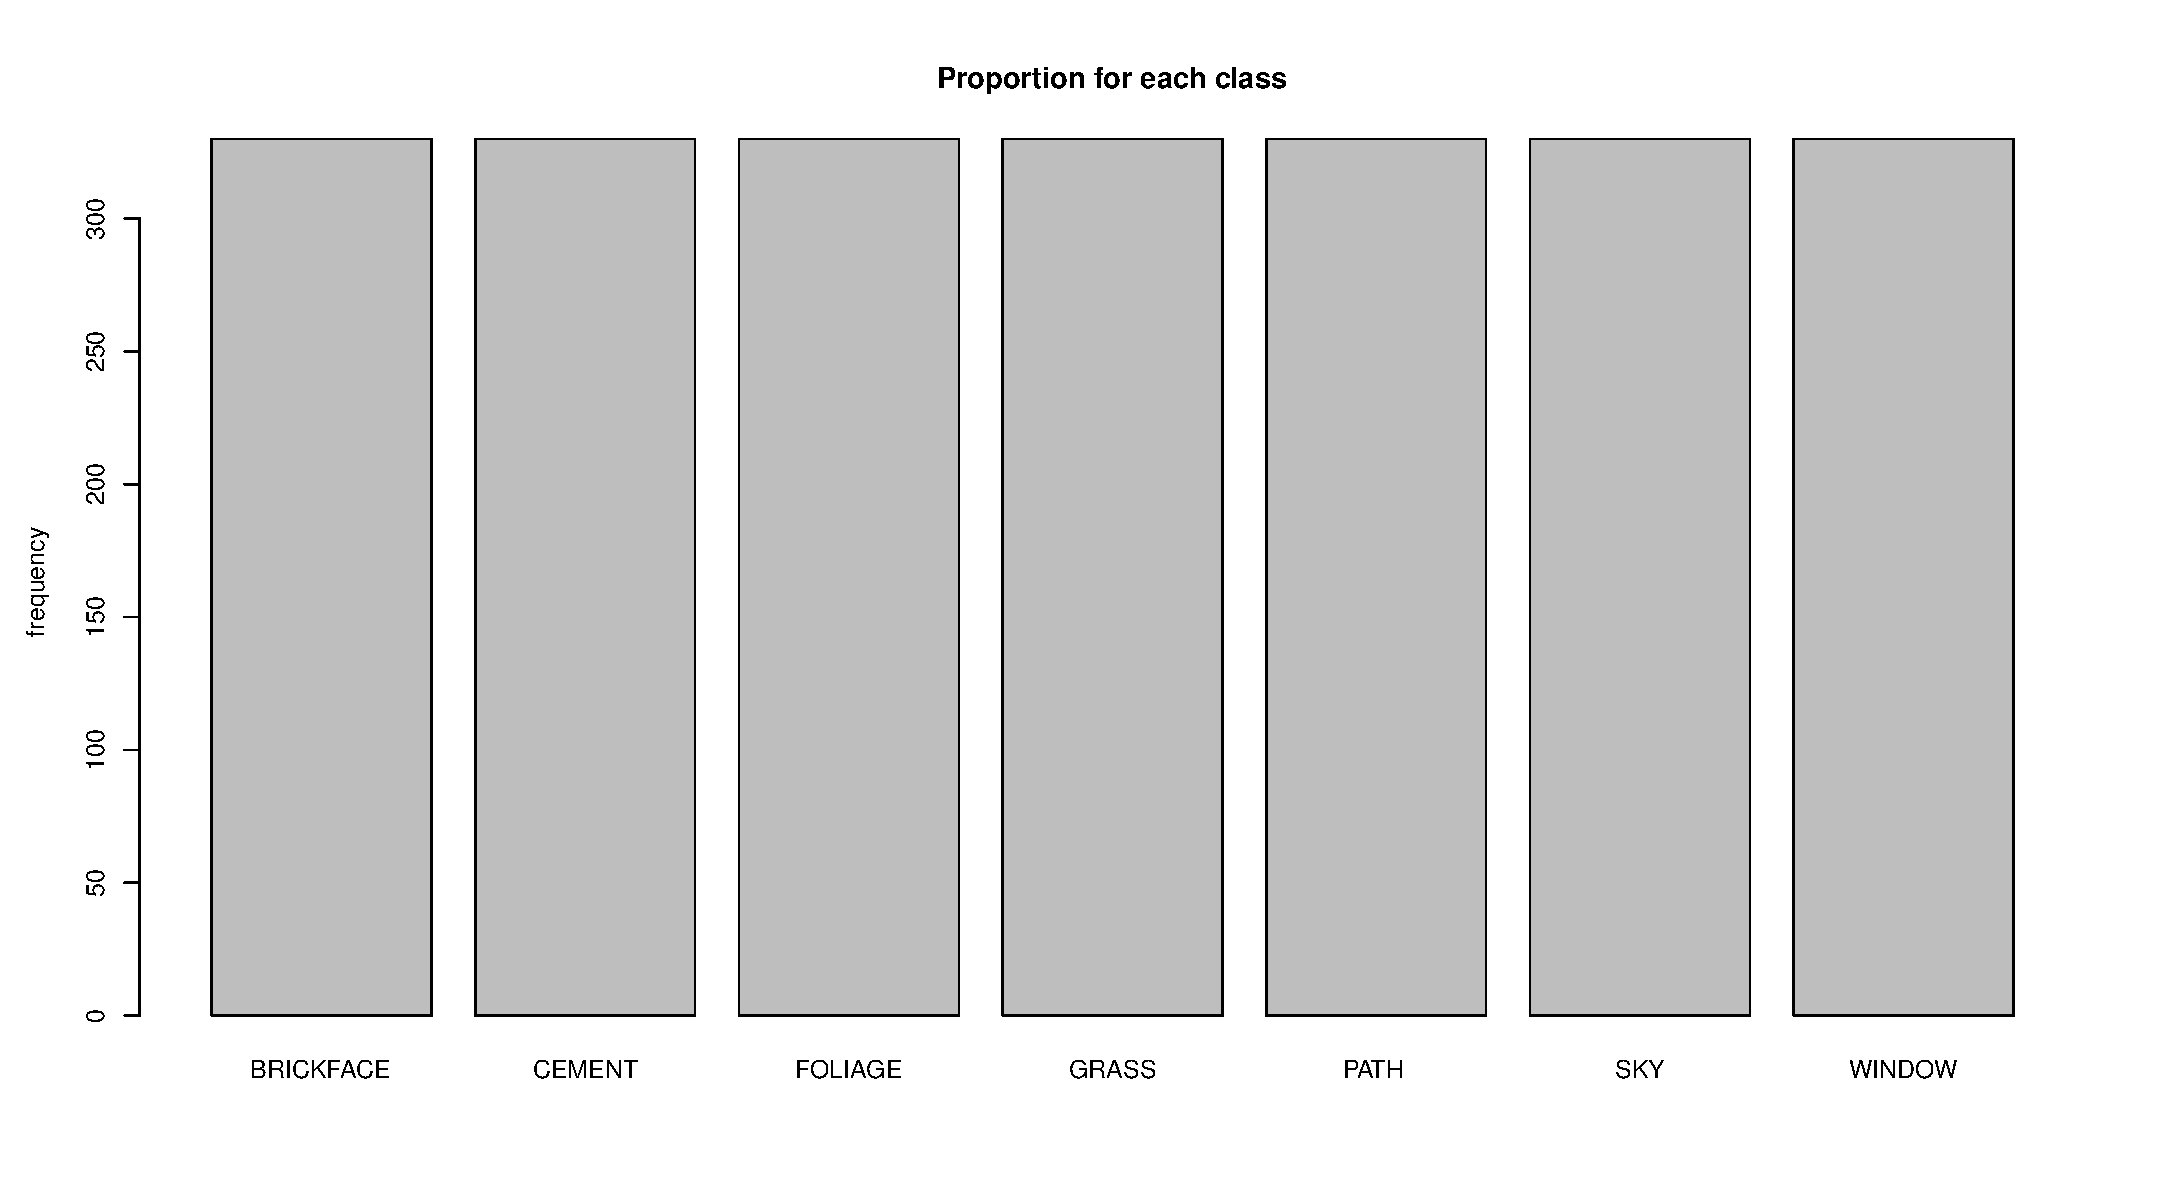
\includegraphics[width=12cm]{class.eps}
\caption{Proportion for classes}
\end{figure}

\begin{figure}[htp]
\centering
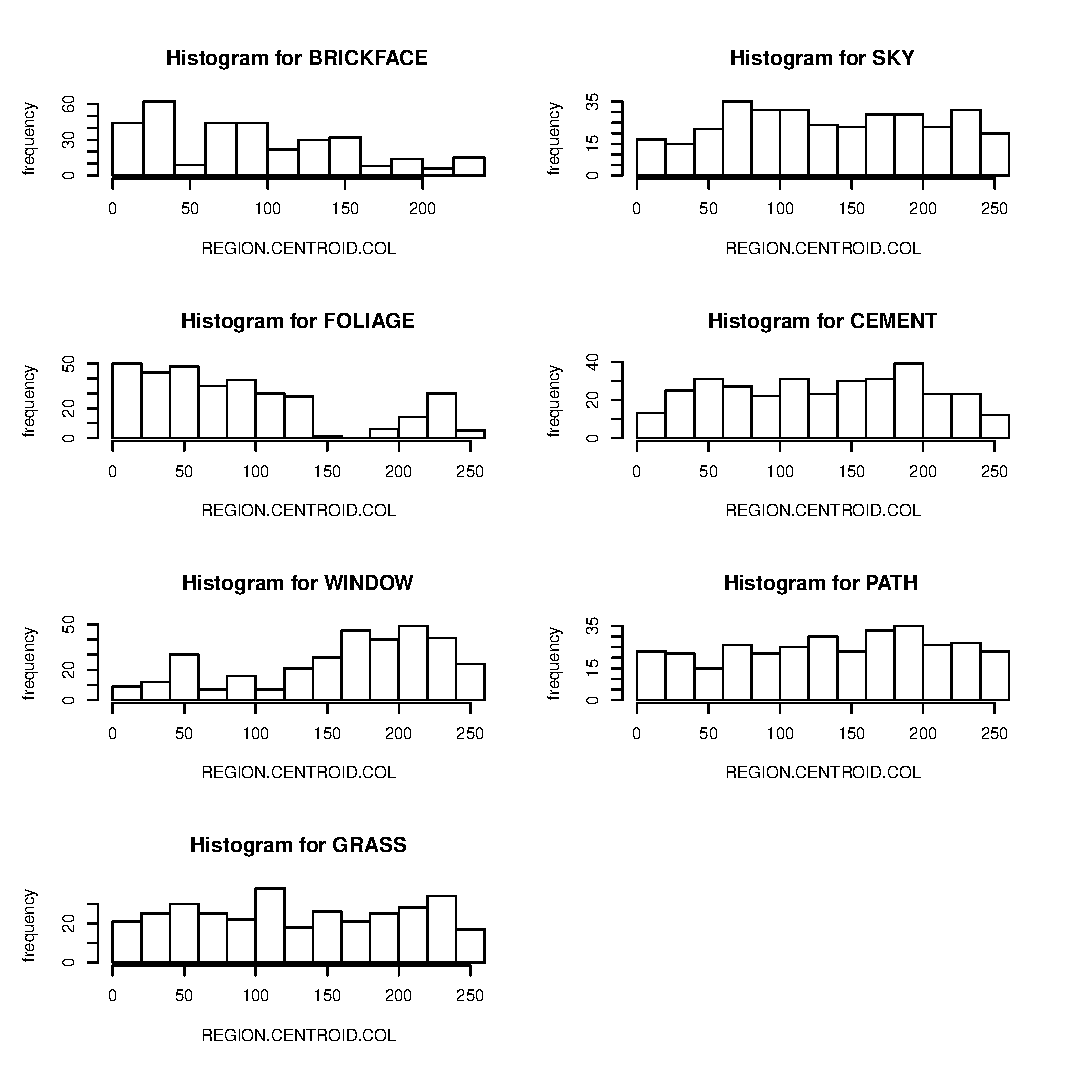
\includegraphics[width=12cm]{a1.eps}
\caption{Histograms for descriptor ``region-centroid-col''}
\end{figure}

\begin{figure}[htp]
\centering
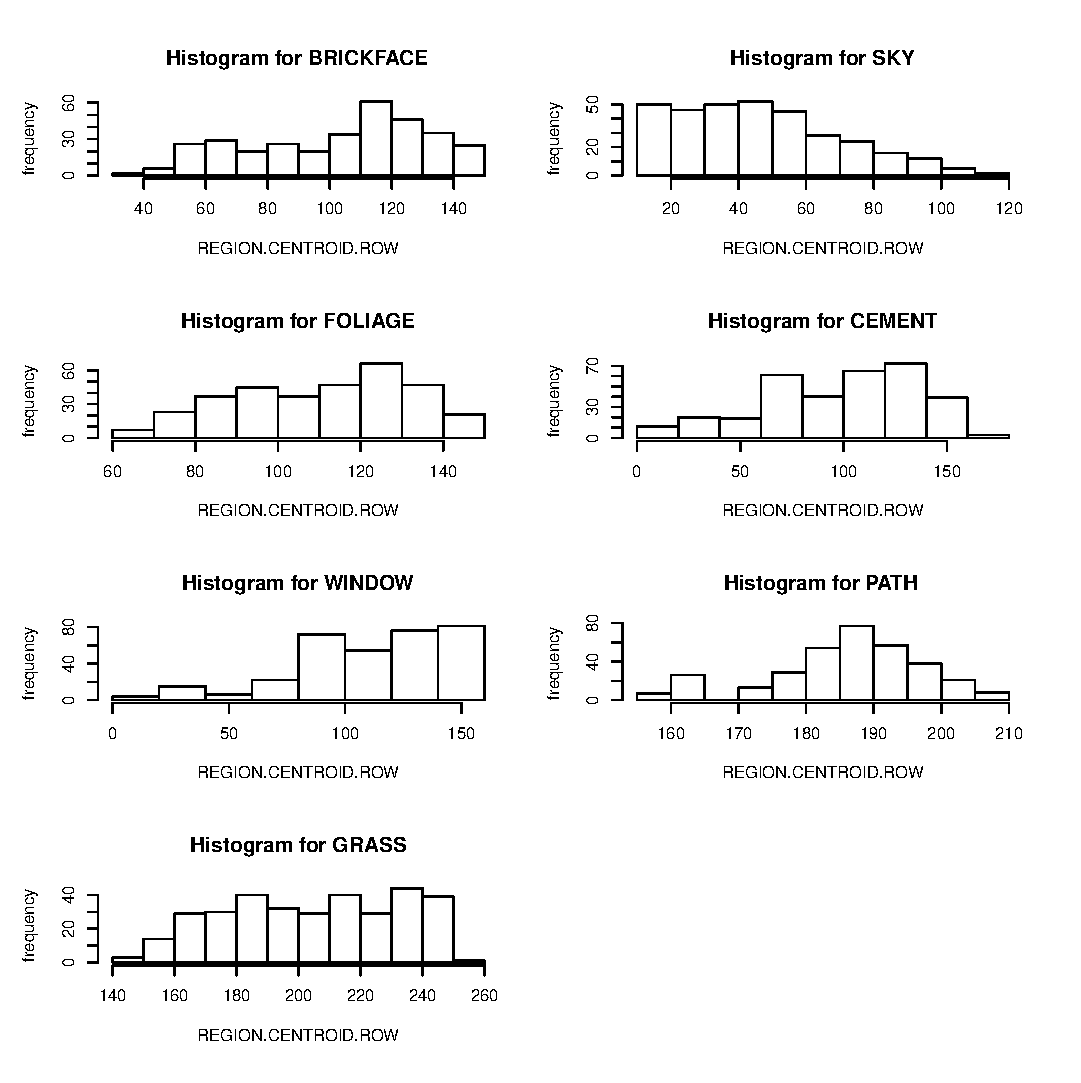
\includegraphics[width=12cm]{a2.eps}
\caption{Histograms for descriptor ``region-centroid-row''}
\end{figure}

\begin{figure}[htp]
\centering
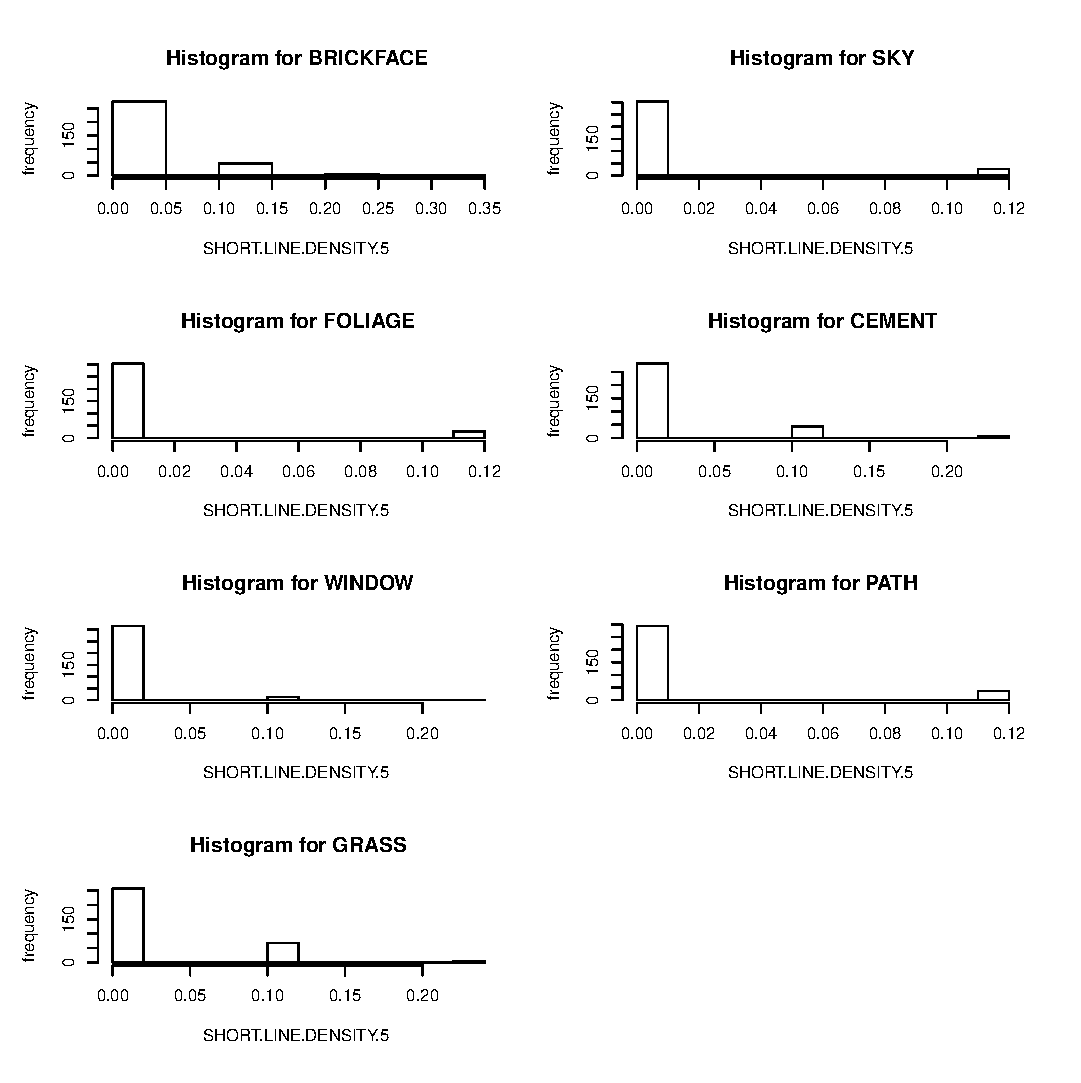
\includegraphics[width=12cm]{a4.eps}
\caption{Histograms for descriptor ``short-line-density-5''}
\end{figure}

\begin{figure}[htp]
\centering
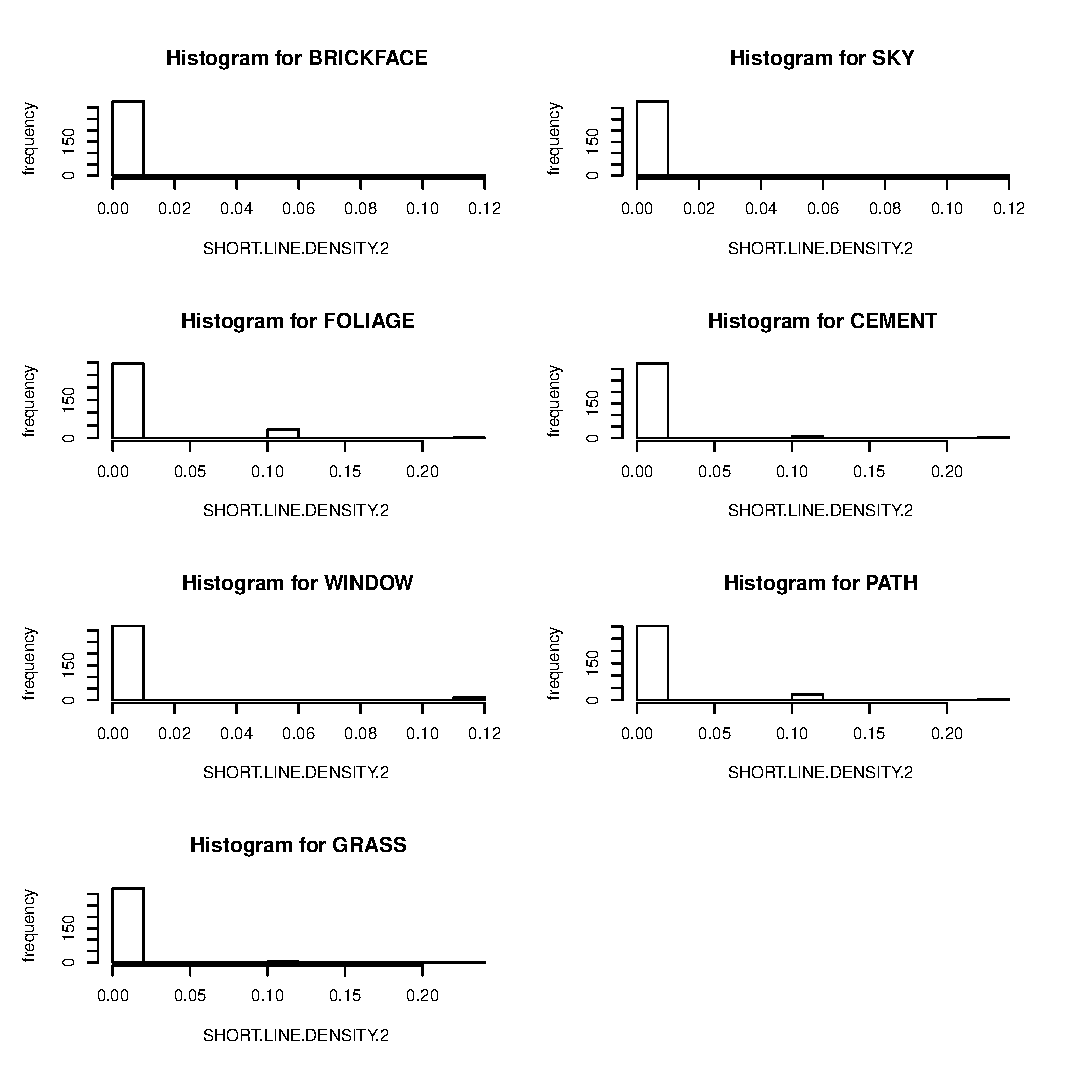
\includegraphics[width=12cm]{a5.eps}
\caption{Histograms for descriptor ``short-line-density-2''}
\end{figure}

\begin{figure}[htp]
\centering
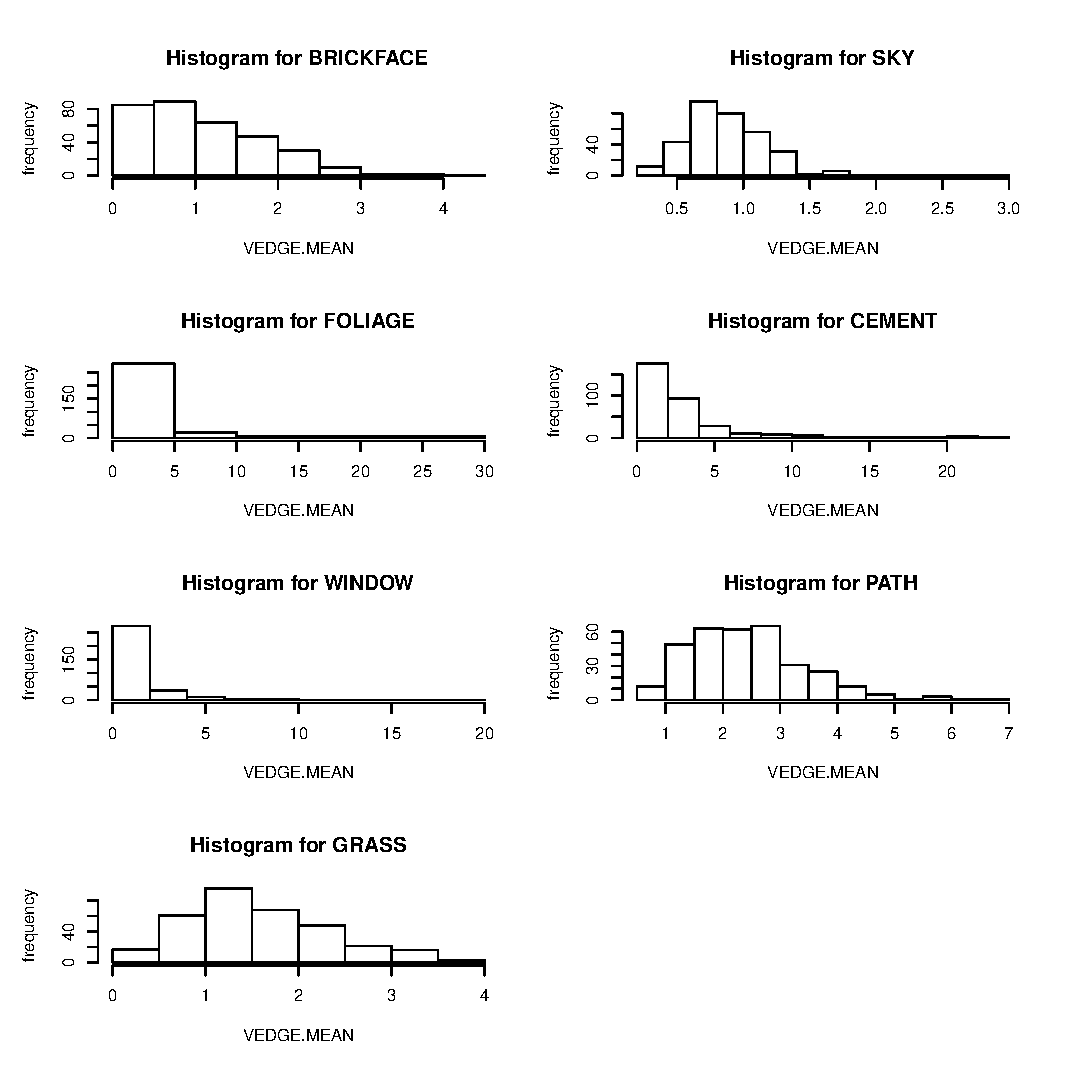
\includegraphics[width=12cm]{a6.eps}
\caption{Histograms for descriptor ``vedge-mean''}
\end{figure}

\begin{figure}[htp]
\centering
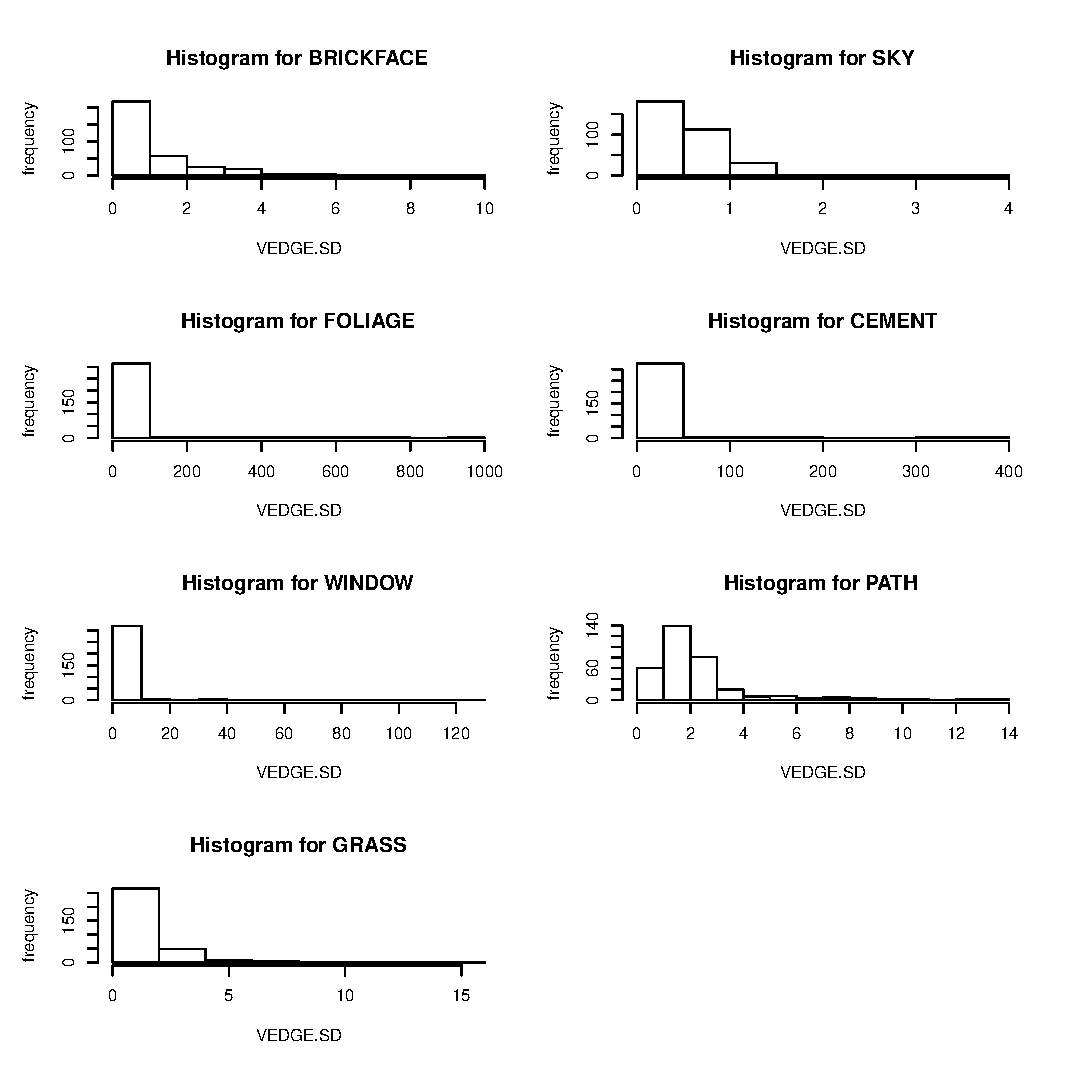
\includegraphics[width=12cm]{a7.eps}
\caption{Histograms for descriptor ``vegde-sd''}
\end{figure}

\begin{figure}[htp]
\centering
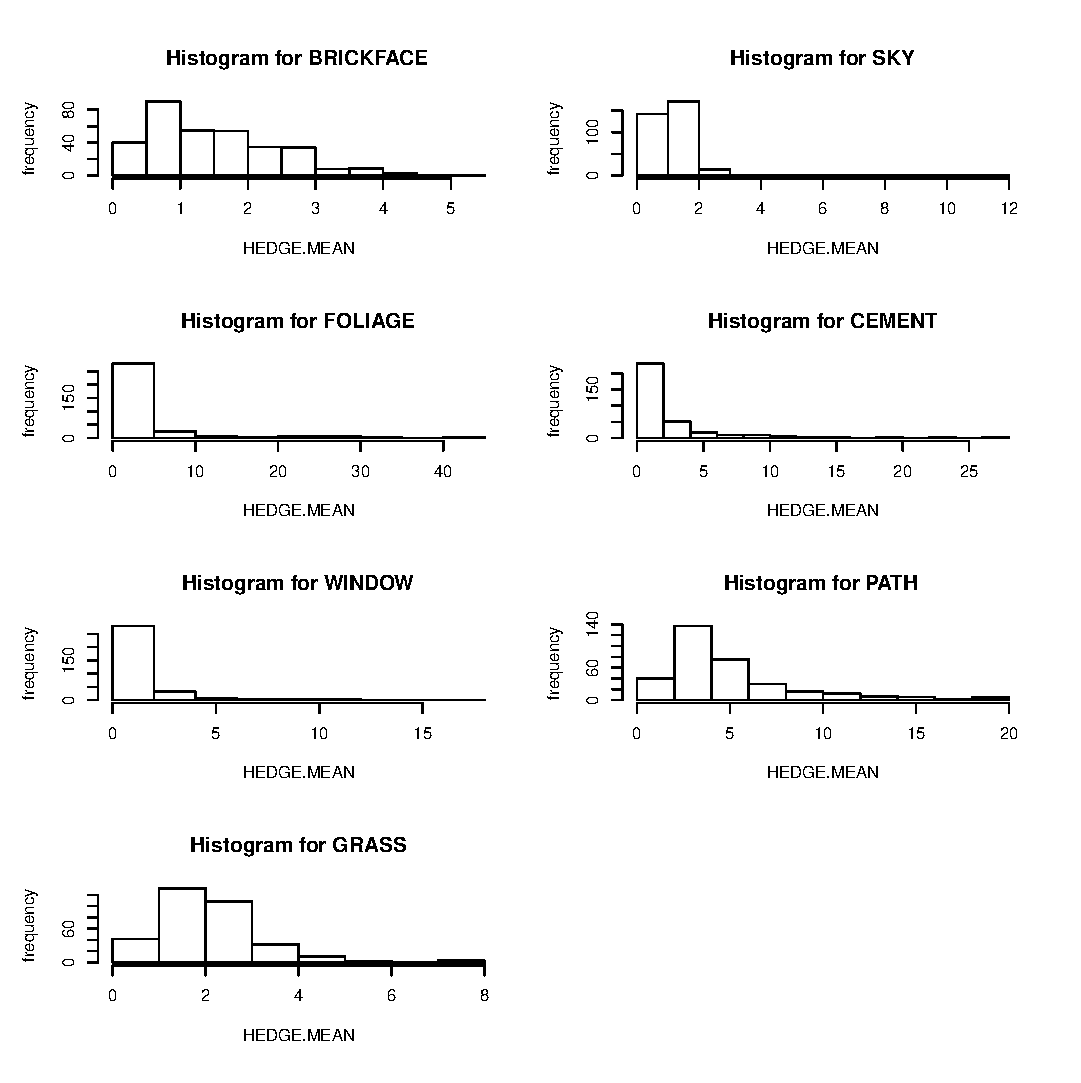
\includegraphics[width=12cm]{a8.eps}
\caption{Histograms for descriptor ``hedge-mean''}
\end{figure}

\begin{figure}[htp]
\centering
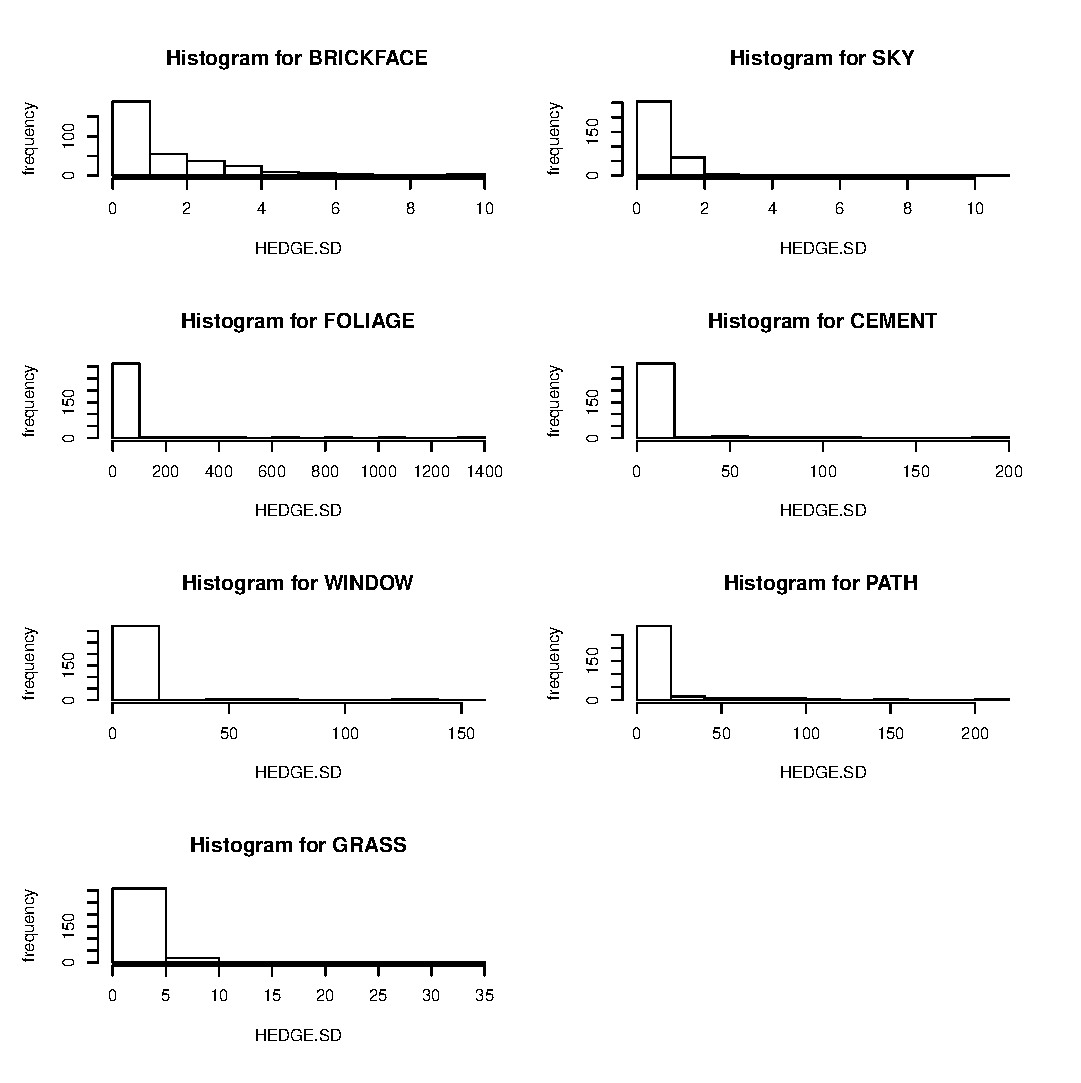
\includegraphics[width=12cm]{a9.eps}
\caption{Histograms for descriptor ``hedge-sd''}
\end{figure}

\begin{figure}[htp]
\centering
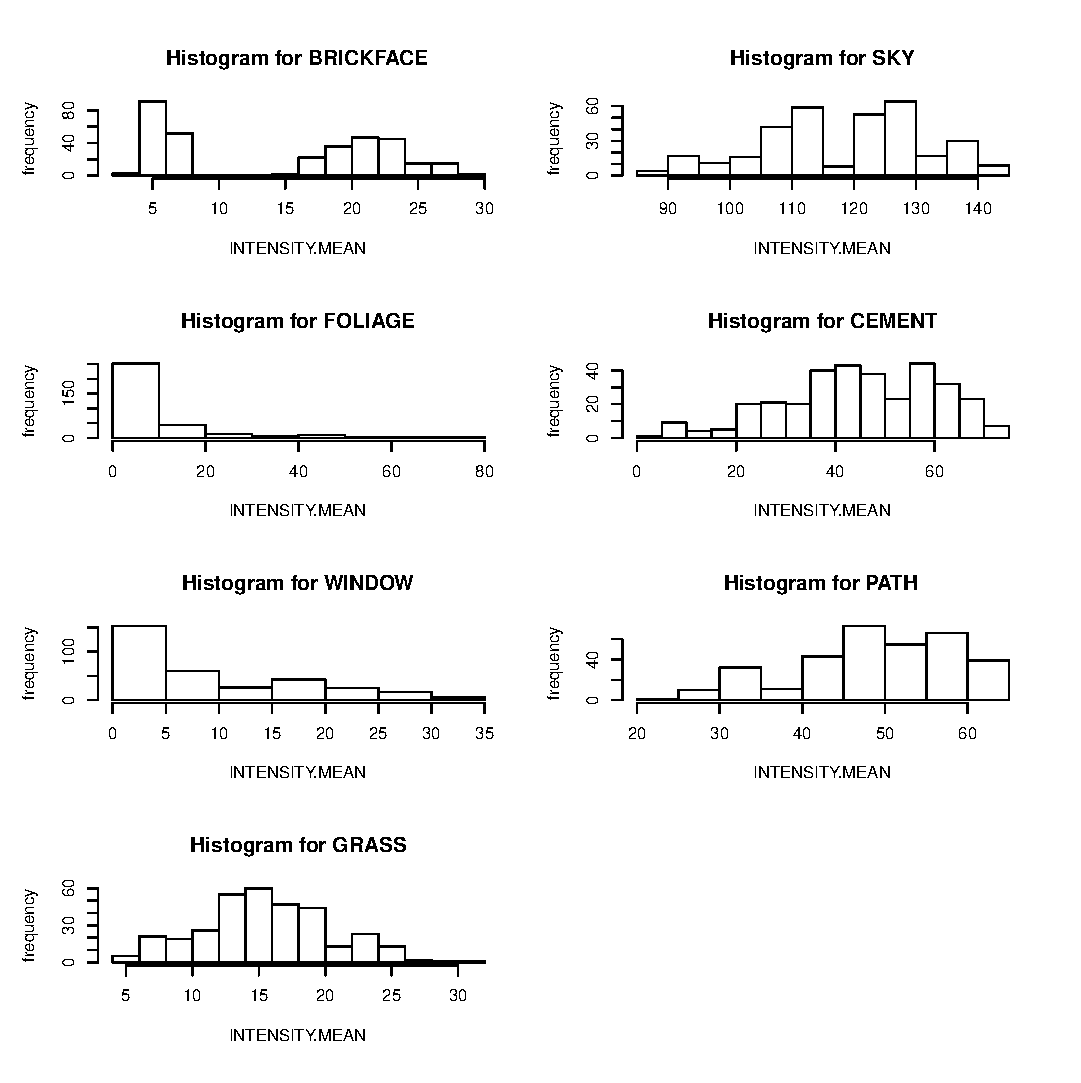
\includegraphics[width=12cm]{a10.eps}
\caption{Histograms for descriptor ``intensity-mean''}
\end{figure}

\begin{figure}[htp]
\centering
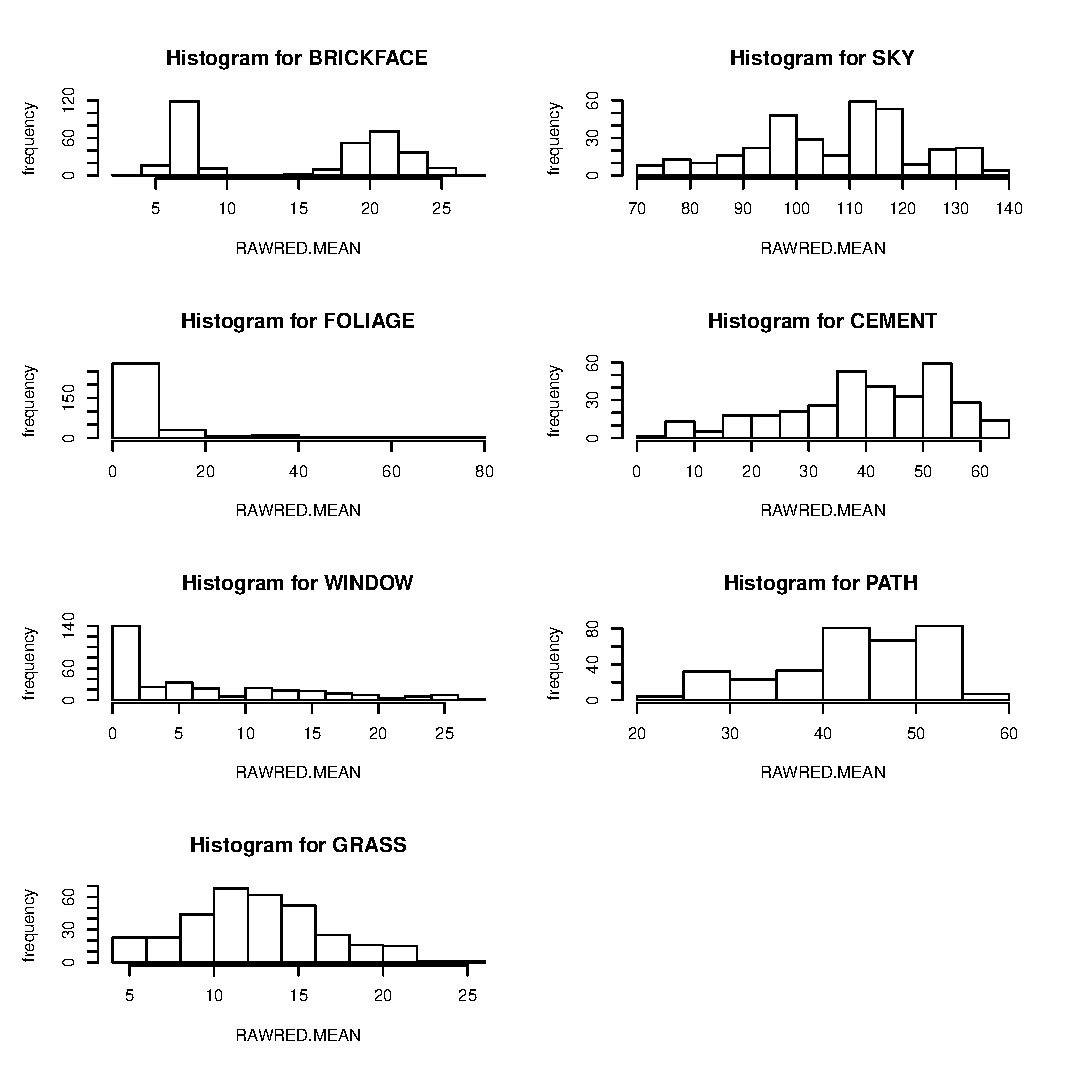
\includegraphics[width=12cm]{a11.eps}
\caption{Histograms for descriptor ``rawred-mean''}
\end{figure}

\begin{figure}[htp]
\centering
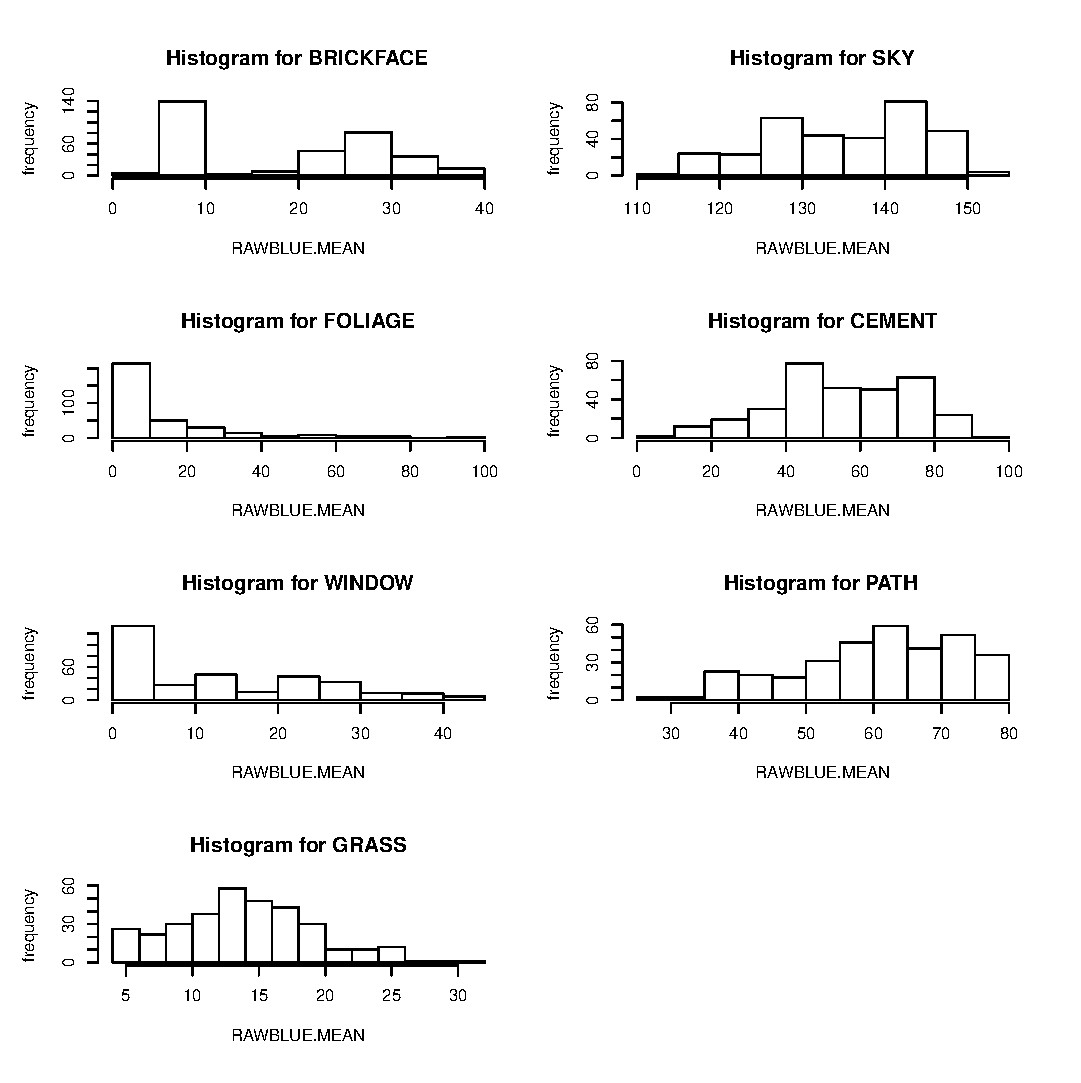
\includegraphics[width=12cm]{a12.eps}
\caption{Histograms for descriptor ``rawblue-mean''}
\end{figure}

\begin{figure}[htp]
\centering
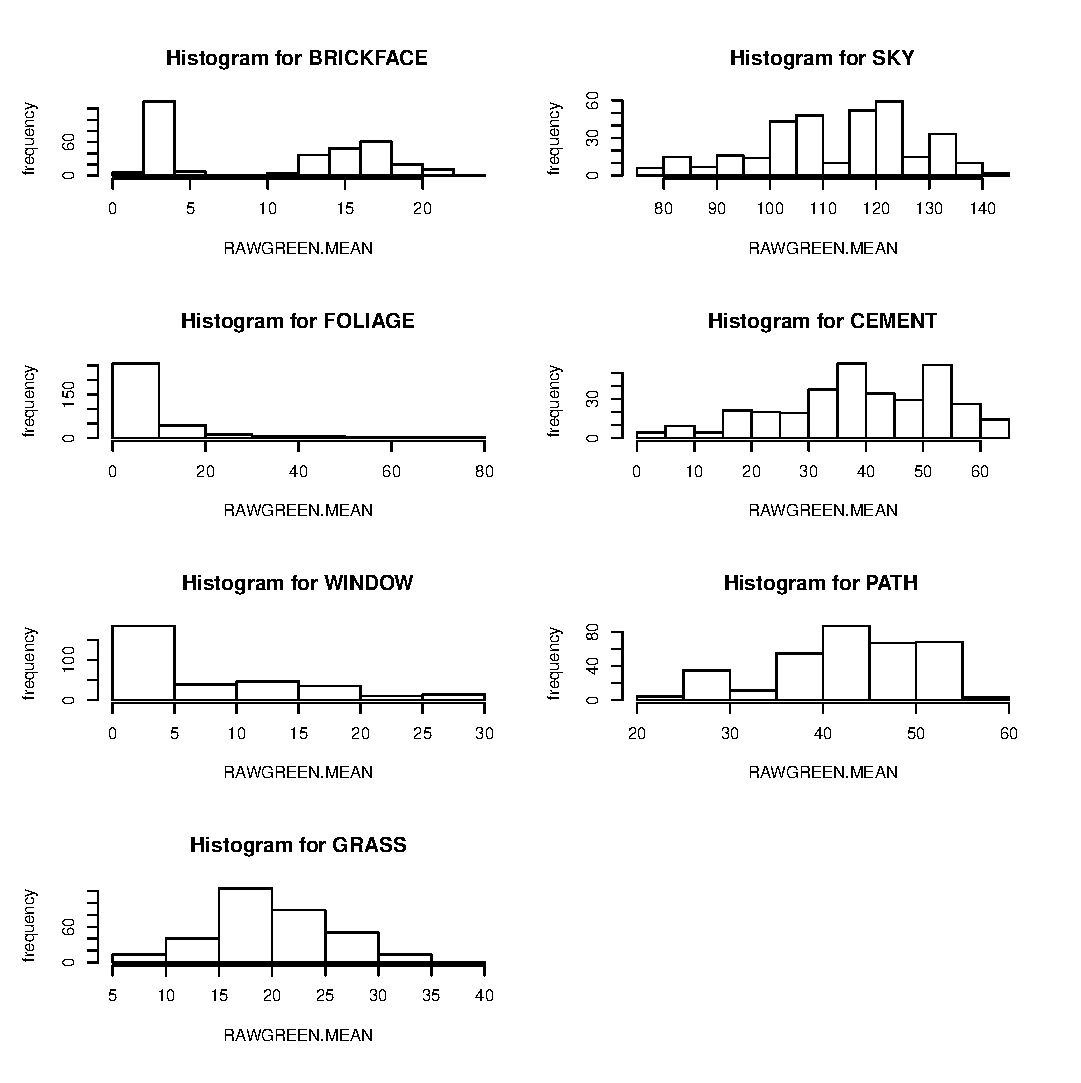
\includegraphics[width=12cm]{a13.eps}
\caption{Histograms for descriptor ``rawgreen-mean''}
\end{figure}

\begin{figure}[htp]
\centering
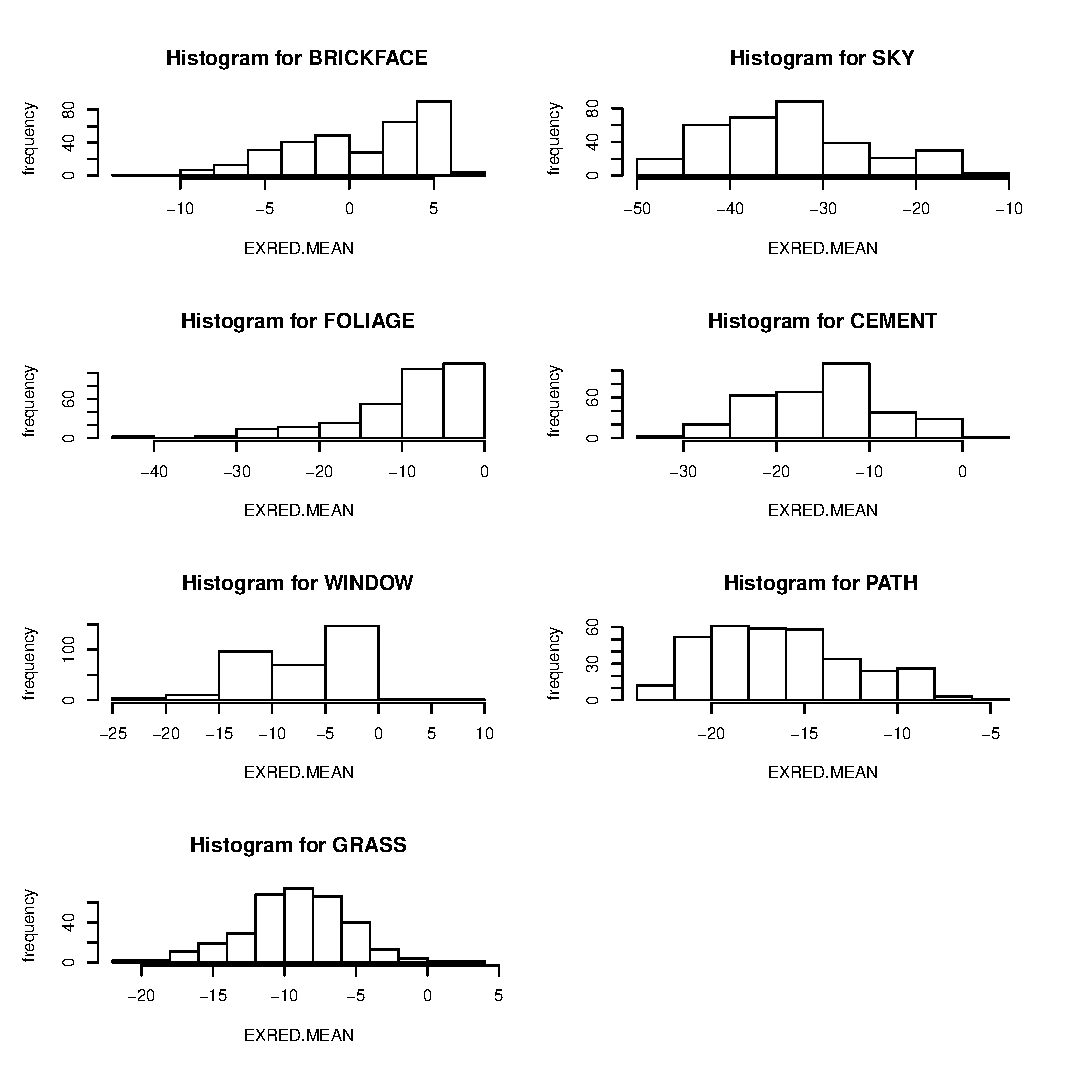
\includegraphics[width=12cm]{a14.eps}
\caption{Histograms for descriptor ``exred-mean''}
\end{figure}

\begin{figure}[htp]
\centering
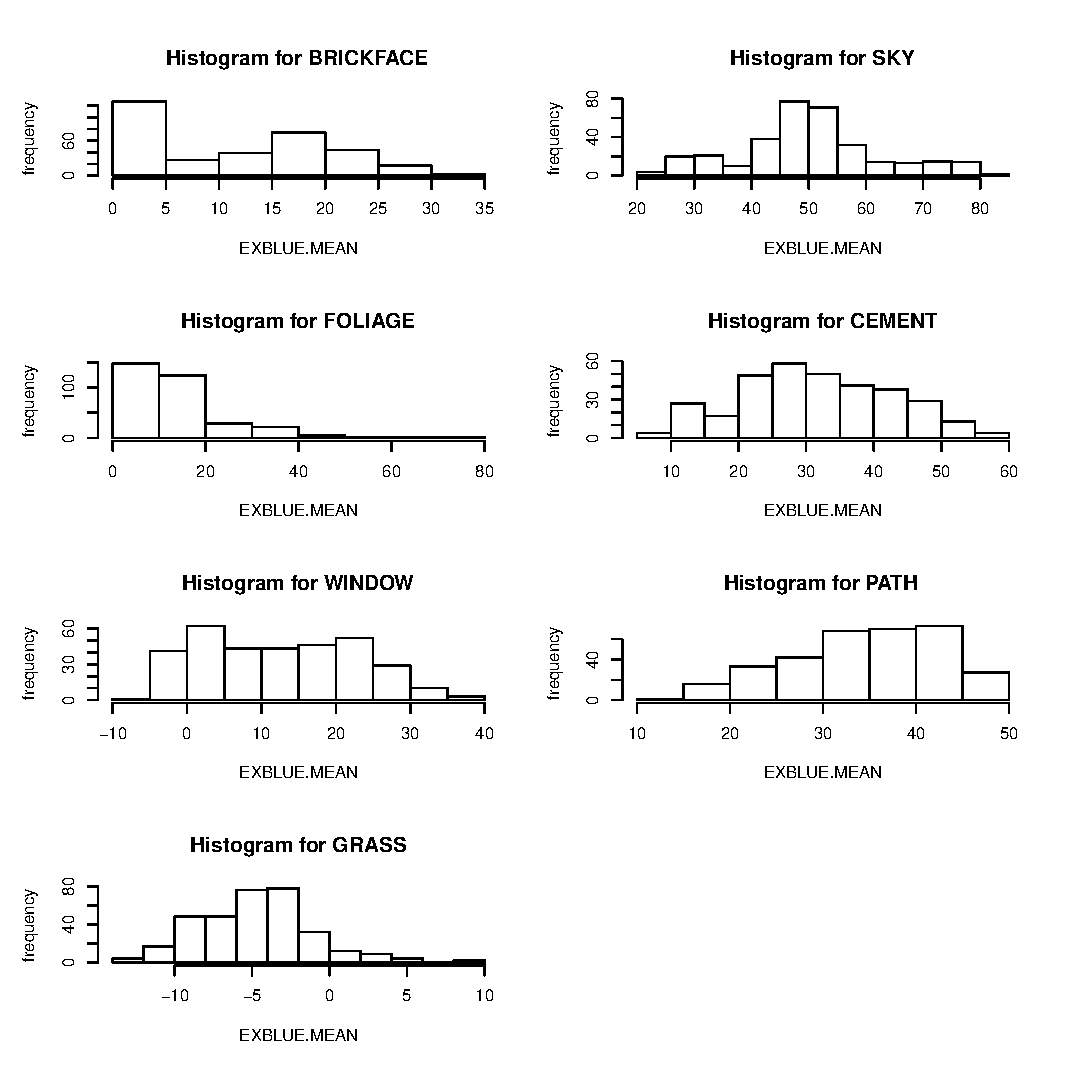
\includegraphics[width=12cm]{a15.eps}
\caption{Histograms for descriptor ``exblue-mean''}
\end{figure}

\begin{figure}[htp]
\centering
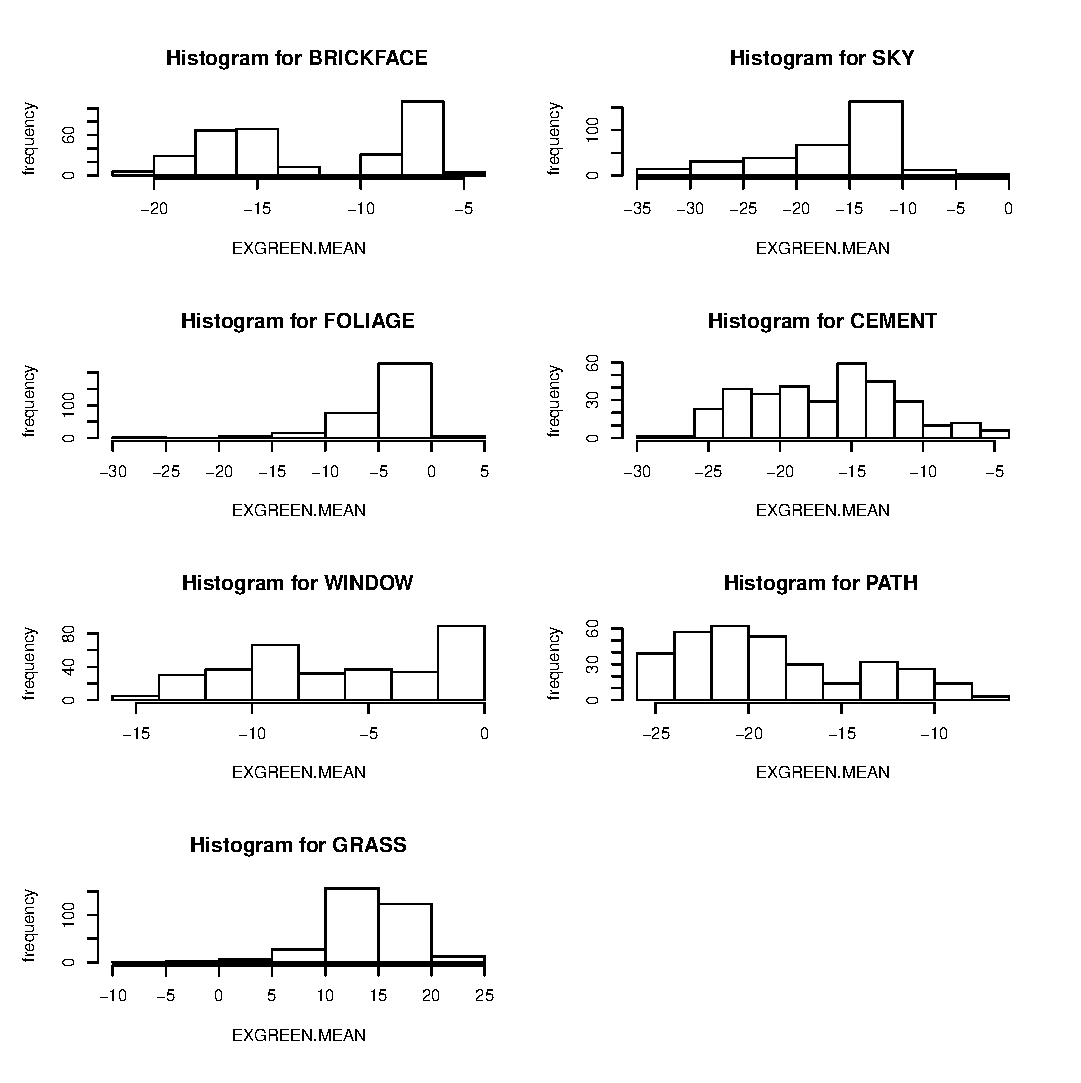
\includegraphics[width=12cm]{a16.eps}
\caption{Histograms for descriptor ``exgreen-mean''}
\end{figure}

\begin{figure}[htp]
\centering
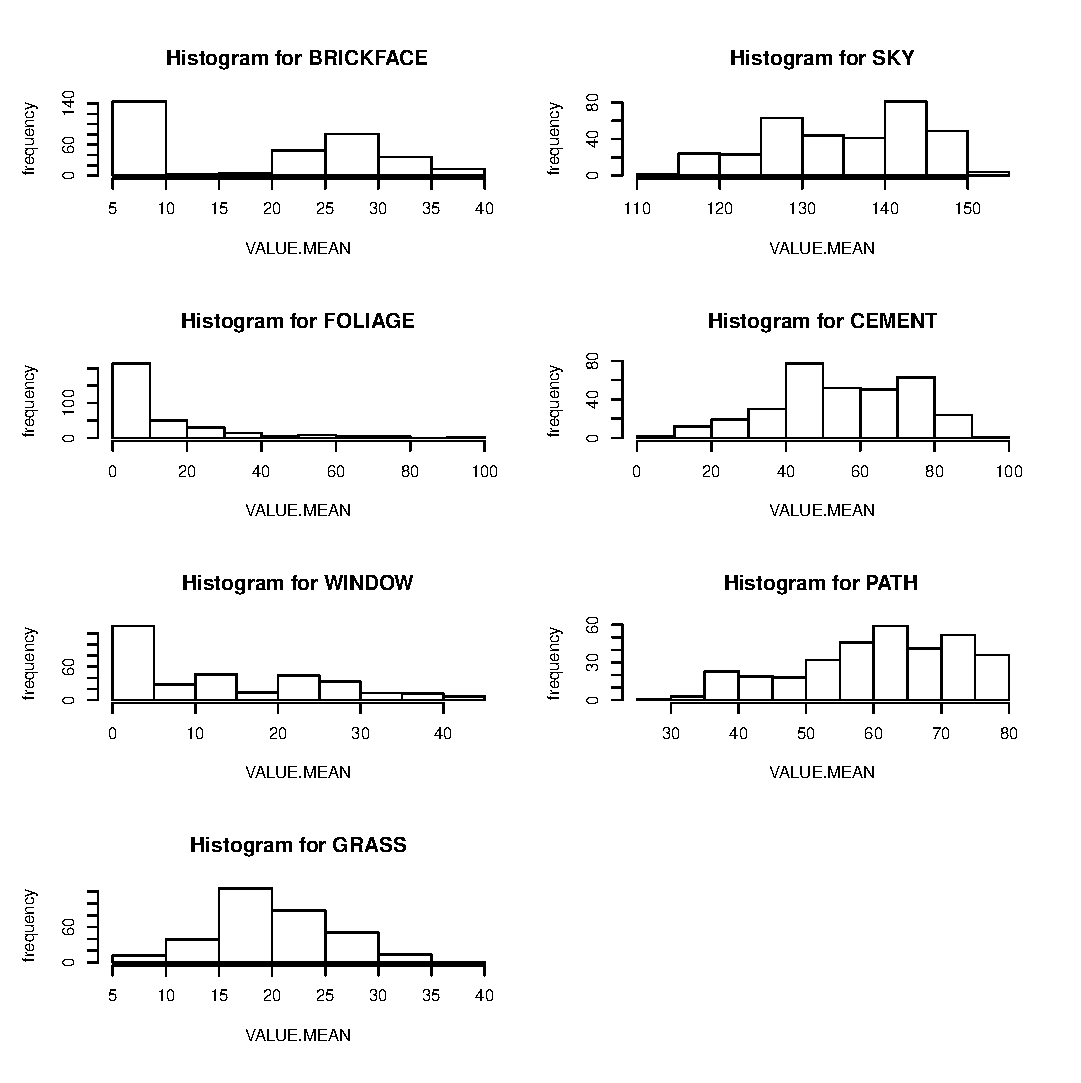
\includegraphics[width=12cm]{a17.eps}
\caption{Histograms for descriptor ``value-mean''}
\end{figure}

\clearpage

\begin{figure}[htp]
\centering
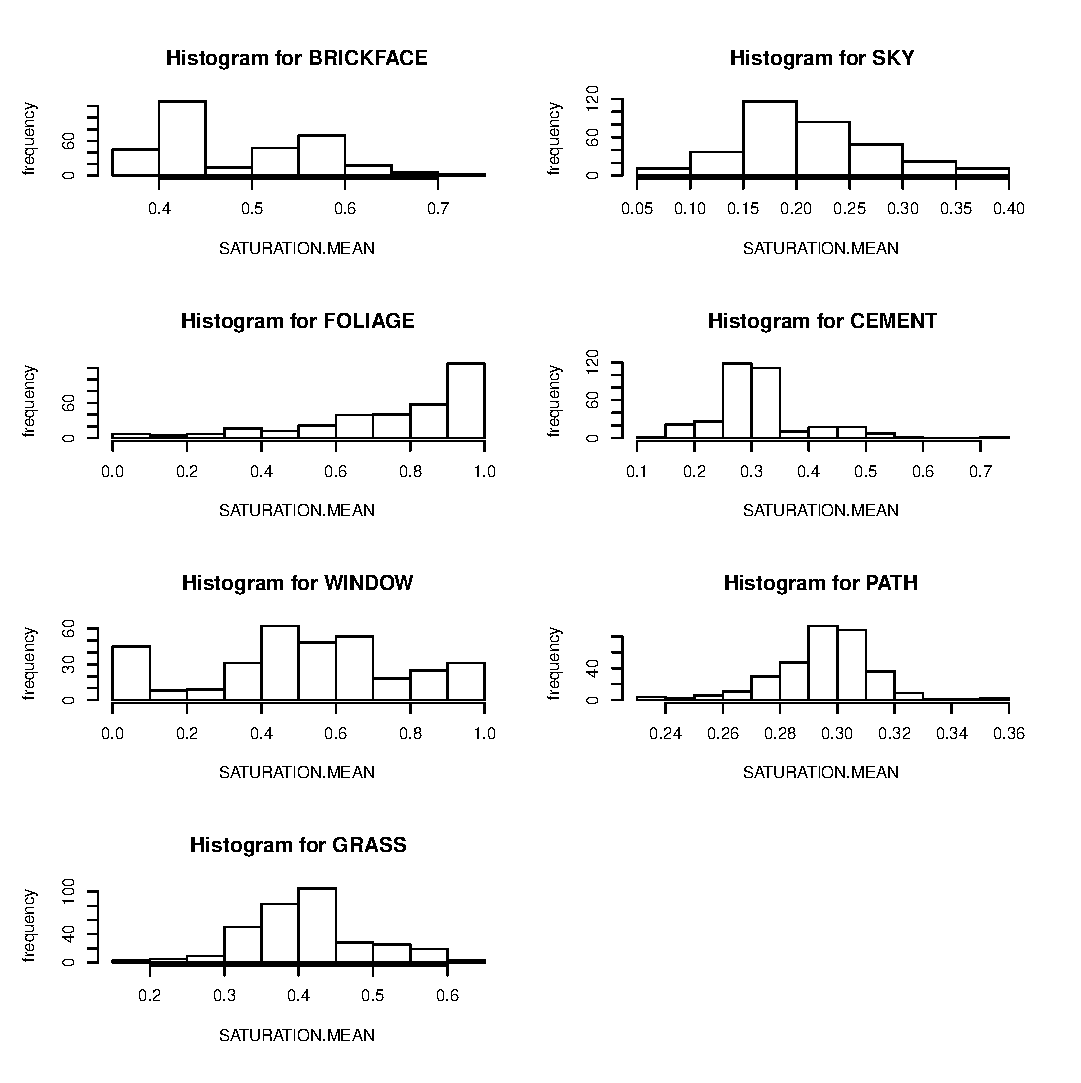
\includegraphics[width=12cm]{a18.eps}
\caption{Histograms for descriptor ``saturatoin-mean''}
\end{figure}

\begin{figure}[htp]
\centering
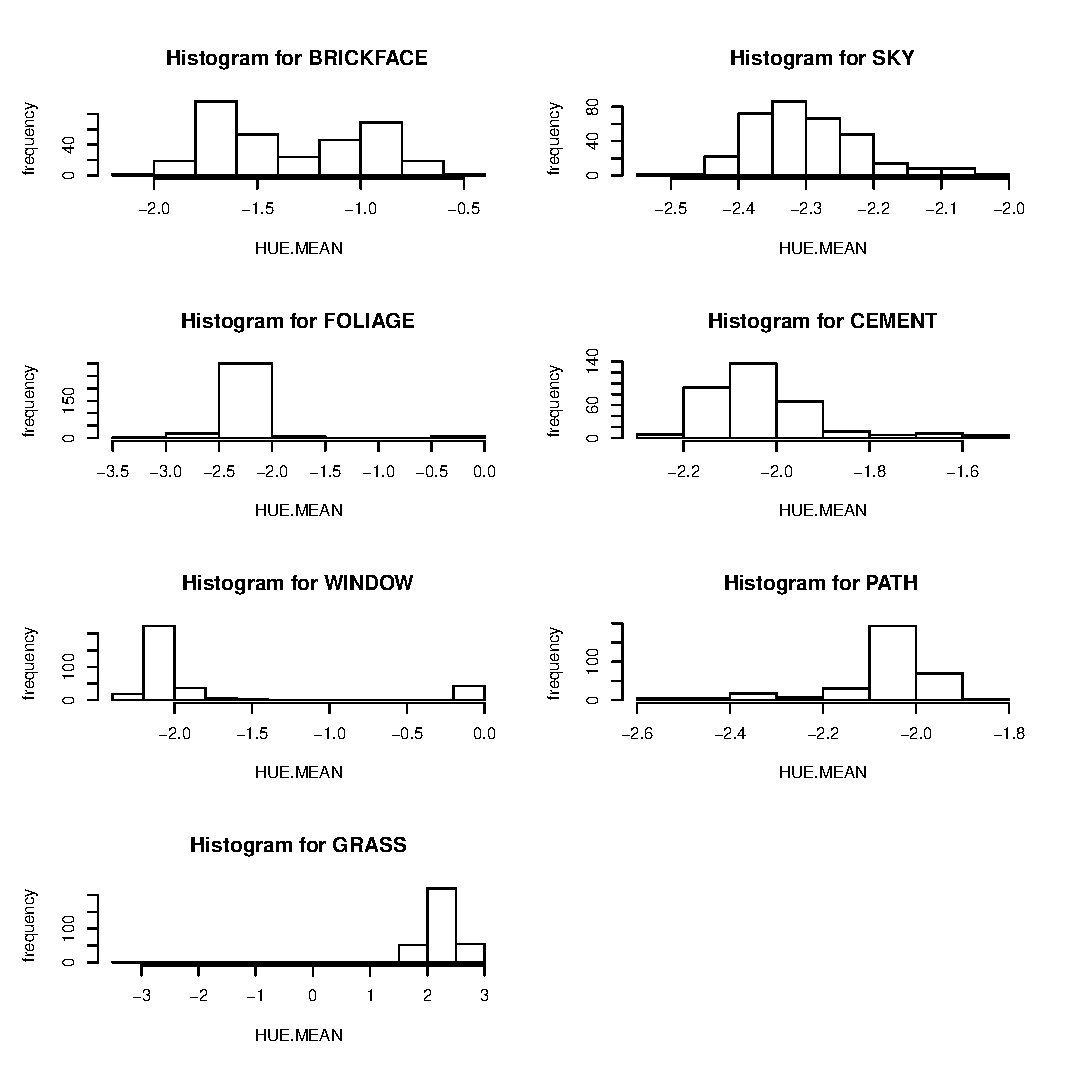
\includegraphics[width=12cm]{a19.eps}
\caption{Histograms for descriptor ``hue-mean''}
\end{figure}




\end{document}


